\documentclass[12pt]{article}
\usepackage[english, portuguese]{babel}
\usepackage[T1]{fontenc}
\usepackage{uarial}
\renewcommand{\familydefault}{\sfdefault}
\usepackage[margin=3cm]{geometry}
\linespread{1.5}
\usepackage{indentfirst}
\setlength\parindent{1.25cm}
\usepackage{tocloft}
\renewcommand{\cftsecleader}{\cftdotfill{\cftdotsep}}
\usepackage{import}
\usepackage[notocbib]{apacite}
\usepackage{multibib}
\newcites{intro}{\centerline{\bfseries\Large References}}
\newcites{review}{\centerline{\bfseries\Large References}}
\usepackage{graphicx}
\usepackage{pdfpages}


\def\blankpage{%
      \clearpage%
      \thispagestyle{empty}%
      \addtocounter{page}{+0}%
      \null%
      \clearpage}

\begin{document}

\renewcommand{\contentsname}{\centerline{\bfseries\Large Table of Contents}}
\tableofcontents

\blankpage

\section*{\hfil Resumo \hfil}
\addcontentsline{toc}{section}{Resumo}
\vspace{1em}

\noindent Acelerómetros são dispositivos que medem as acelerações do corpo e têm sido amplamente adotados para monitorar atividade física. O seu uso mais frequente é determinar o gasto energético (GE) e a intensidade da atividade física (IAF), mas mais recentemente começaram a ser explorados como um meio de estimar a carga mecânica esquelética. No entanto, quase todos os estudos de calibração de acelerómetros foram desenvolvidos para pessoas não obesas, o que prejudica a aplicação de seus resultados nos obesos. Portanto, o objetivo geral deste trabalho foi o de melhorar a precisão da predição do GE e da carga mecânica e da classificação da IAF, especialmente em pacientes obesos. Para isso, o presente trabalho está estruturado em: i) uma revisão de literatura sobre os acelerómetros, seu processo de calibração e sua utilização para predizer o GE e a carga mecânica; ii) um artigo original que objetivou desenvolver equações de regressão para predizer o GE e pontos de corte para classificar a IAF em pessoas obesas severas baseado em várias métricas de aceleração; e iii) um artigo original que objetivou desenvolver equações baseadas em acelerometria para predizer o pico da força de reação do solo (pFRS) em sujeitos de peso normal até obesos severos. Os resultados revelaram que todos os modelos de predição desenvolvidos para o GE e o pFRS e os pontos de corte para classificar a IAF apresentaram uma boa precisão, com resultados similares ou melhores comparados a outros estudos prévios. Em conclusão, os dados de acelerometria permitem predizer precisamente o GE e classificar a IAF em obesos severos e predizer o pFRS em sujeitos de peso normal até obesos severos. Portanto, futuros estudos podem adotar equações de regressão e pontos de corte apropriadamente desenvolvidos para os obesos e também facilmente determinar a intensidade da carga mecânica in condições clínicas com a utilização de acelerómetros.

\vspace{\fill}
\noindent
\textbf{Palavras-chave:} MONITORES DE ATIVIDADE, OBESIDADE, VALIDAÇÃO, CALORIMETRIA INDIRETA, CARGA MECÂNICA

\blankpage

\section*{\hfil Abstract \hfil}
\addcontentsline{toc}{section}{Abstract}
\vspace{1em}

\noindent Accelerometers are small wearable devices that measure body accelerations and have been widely adopted to objectively monitor physical activity. Their most frequent use is to determine energy expenditure (EE) and physical activity intensity (PAI), but more recently they have started to be explored as a way to estimate skeletal mechanical loading. However, almost all accelerometer calibration studies were developed for non-obese people, hindering an accurate prediction of EE and mechanical loading, as well as inducing a misclassification of PAI in obese patients. Therefore, the general aim of this work was to improve the accuracy of EE and mechanical loading prediction and PAI classification, specially in obese patients. For this, the current work is structured in: i) a literature review about accelerometers, their calibration process and their use to predict EE and mechanical loading; ii) an original article which aimed to develop regression equations to predict EE and cut-points to classify PAI in severely obese people based on several accelerometry metrics; and iii) an original article which aimed to develop accelerometry-based equations to predict peak ground reaction forces (pGRF) on normal weight to severely obese subjects. The results revealed that all of our prediction models developed for EE and pGRF prediction and our cut-points for PAI classification presented a good accuracy with similar or better results compared to other previously published studies. In conclusion, accelerometry data allow to accurately predict EE and classify PAI in severely obese people and to predict pGRF in normal weight to severely obese subjects. Therefore, future studies may adopt appropriate regression equations and cut-points developed for obese people and also to easily determine mechanical loading intensity in clinical settings using accelerometers.

\vspace{\fill}
\noindent
\textbf{Keywords:} ACTIVITY MONITOR, OBESITY, VALIDITY, INDIRECT CALORIMETRY, MECHANICAL LOADING
\pagebreak


\section*{\vfill\raggedleft\bfseries 1. General introduction}
\addcontentsline{toc}{section}{1. General introduction}
\thispagestyle{empty} 
\pagebreak

\section*{General introduction}

There are plenty of evidence supporting the role of physical activity (PA) in health improvement and chronic diseases prevention \citeintro{Guthold_2018, Warburton_2017, Warburton_2006}. These evidences contributed to the emergence of recommendations about the type, amount and intensity of PA necessary to maintain  or improve health in the general population \citeintro{WHO_2010}, and also led to the need of accurate methods to assess PA during daily living \citeintro{Montoye_2000, Plasqui_2013} either subjectively or objectively. Accelerometers are among the most common devices to objectively measure PA \citeintro{Strath_2013}, but as they only measure the body segment accelerations, their output needs to be translated into more biologically meaningful information by a process called calibration \citeintro{Welk_2005}.
 
Nowadays, the majority of calibration studies use the accelerometer output to determine some cardio-metabolic parameters such as energy expenditure (EE) and PA intensity (PAI) levels \citeintro{Migueles_2017}, but among other important uses is the estimation of biomechanical parameters, such a ground reaction force \citeintro{Neugebauer_2014}. Another important aspect of the accelerometer calibration studies is that their application is only valid for a population similar to those of the utilised sample \citeintro{Welk_2005}. Obese people present some different characteristics than the non-obese, as a low resting metabolic rate \citeintro{Byrne_2005}, lower aerobic physical fitness \citeintro{Souza_2010} and some biomechanical gait alterations \citeintro{Bode_2019}. As obesity is an increasingly prevalent condition \citeintro{Guthold_2018}, specific accelerometer calibration studies are needed for this population in order to accurately estimate the PA related parameters to be used to monitor PA, exercise and their effects on health.

Therefore, the purposes of this work were, first, to develop regression equations to predict EE and cut-points to classify sedentary activity and PAI in severely obese people based on several metrics obtained from accelerometer data; and second, to develop accelerometry-based equations to predict peak ground reaction forces (pGRF) on normal weight to severely obese subjects. In order to attend this goal, this dissertation is structured in four chapters. The first chapter consists of the general introduction, which presented some background information concerning the dissertation main theme and the primary objectives. The second chapter includes a literature review about accelerometers, their calibration process and their use to predict EE and skeletal mechanical loading. The third chapter is composed of two original articles that developed accelerometry-based prediction models to EE and cut-points to classify PAI and also several regression equations to predict pGRF using raw accelerometer data on normal weight to severely obese subjects. Finally, the fourth chapter presents the dissertation general conclusions and future perspectives.

\pagebreak

\bibliographyintro{bibliography}
\bibliographystyleintro{fadeup}
\pagebreak


\section*{\vfill\raggedleft\bfseries 2. Literature review}
\addcontentsline{toc}{section}{2. Literature review}
\thispagestyle{empty} 
\pagebreak

\section*{Introduction}

Physical activity (PA) has long been established as one of the main contributors to prevent chronic diseases and promote health \citereview{Kaminsky_2014, Warburton_2017}. Evidence shows that lack of PA leads to an increased risk of cardiovascular disease, diabetes, hypertension, osteoporosis, several types of cancer and a higher mortality risk \citereview{Guthold_2018, Lee_2012, Shiroma_2014}. Given the relevant relationship between PA and health, there is an increasing need of accurate and reliable methods of PA assessment on daily life \citereview{Montoye_2000, Plasqui_2013, Strath_2013}. These methods can be either subjective, such as questionnaires, or objective, as direct observation and wearable devices \citereview{Strath_2013, Troiano_2005}.

The most commonly used wearable devices to assess PA are accelerometers \citereview{Strath_2013}. These are equipments that detect the body movement accelerations in one to three orthogonal planes (anteroposterior, mediolateral, and vertical) \citereview{Chen_2005}. The accelerometers output can be either raw acceleration, usually expressed as gravitational acceleration units (\textit{g}), or activity counts (AC), which are processed data derived from the raw acceleration and are based on manufacturer-specific algorithm \citereview{Chen_2005, Basset_2012, Troiano_2014}. In both cases, the accelerometer output needs to be translated into more biologically meaningful information through a calibration process \citereview{Matthews_2005}.

Currently, most calibration studies use the accelerometer output to determine energy expenditure (EE) and PA intensity levels \citereview{Migueles_2017, Mendes_2018} but they can be also used to estimate biomechanical parameters, such as ground reaction forces (GRF) \citereview{Neugebauer_2014, Fortune_2014}, to evaluate standing balance \citereview{Mayagoitia_2002}, to detect the type of PA being performed \citereview{Bonomi_2009, Zhang_2012}, among others. Apart from the standard measure against which the accelerometer output needs to be compared, calibration studies must carefully define the sample characteristics, PA protocols and statistical approaches, as these aspects can greatly influence the study internal and external validity \citereview{Basset_2012, Welk_2005}. This led to the emergence of several different calibration studies in the literature with distinct methods to predict a given outcome variable \citereview{Mendes_2018, Matthews_2018}.

This current review aims to describe the literature regarding the use of accelerometers to measure EE, classify PA intensities and estimate GRF, as well as issues about calibration and validation studies of these wearable monitors. 

\section*{Accelerometers}

As said previously, accelerometers are wearable devices used to measure PA related variables \citereview{Chen_2005}. The first portable accelerometer was developed in the 1980s \citereview{Wong_1981, Montoye_1983} and with the many technological advances since then, the use of such devices in research is ever growing, with a major increase in the number of published articles mentioning PA or exercise and accelerometers since the early 2000s (Figure \ref{art_year}).

\begin{figure}[h]
	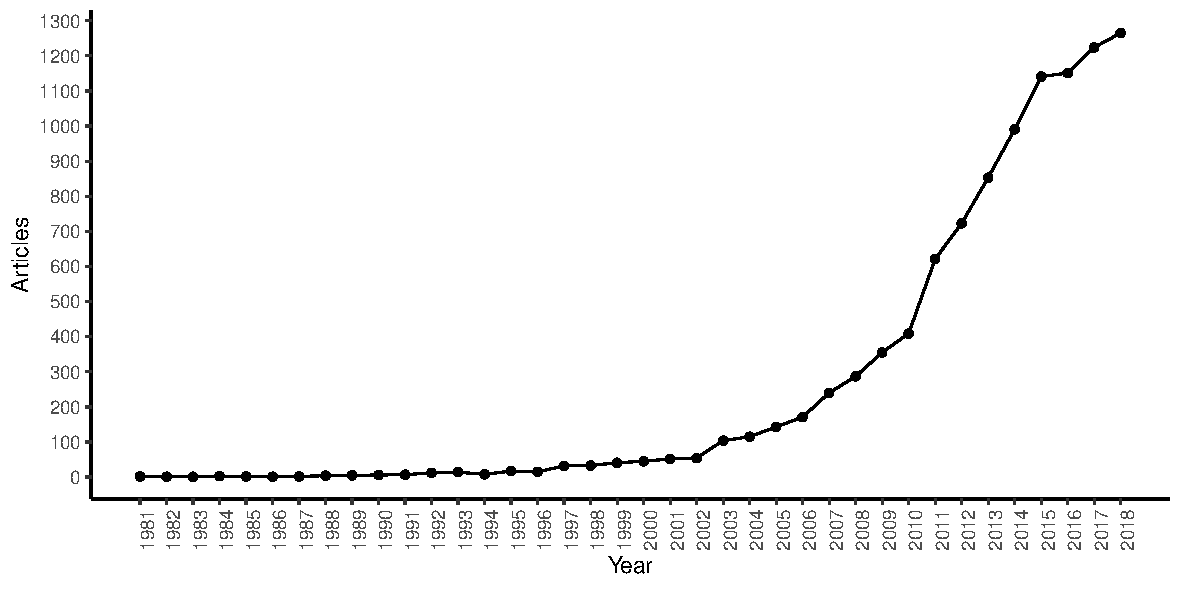
\includegraphics[width=\linewidth]{figs/fig1.pdf}
	\caption{Articles published by year with search terms ``exercise or physical activity'' and ``accelerometer or accelerometry'', Scopus.com, accessed 15 April 2019.}
	\label{art_year}
\end{figure}

From a technical standpoint, the working principle of most accelerometers is based on a sensing element, the seismic mass, and a piezoelectric element. When this system suffers an acceleration, the seismic mass causes a deformation in the piezoelectrical element, generating an output voltage signal proportional to the applied acceleration \citereview{Chen_2005, Yang_2010}. The rate by which this data is acquired is determined by the sampling frequency of the device, making it responsive not only to the acceleration intensity, but to its frequency \citereview{Mathie_2004}. The signal is then filtered and processed before being digitally stored by the equipment \citereview{Chen_2005}.

As an objective method to measure PA, accelerometers offer some advantages over subjective methods, such as questionnaires and PA diaries. They are capable of long term continuous data collection with low subject burden \citereview{Chen_2012, Strath_2013}, are more accurate than questionnaires to measure PA and sedentary behaviour \citereview{Celis-Morales_2012, Matthews_2018} and can measure the full spectrum of daily activities, providing more detailed intensity, frequency and duration data \citereview{Matthews_2018, Strath_2013}.

On the other hand, accelerometers also present some weaknesses. They cannot reliably account for some activities, such as cycling, climbing stairs, weight-lifting and upper-body activities when worn at hip or lower back \citereview{Strath_2013}. Also, different manufacturers have distinct proprietary algorithms to compute raw data into AC, hindering the comparison of the accelerometer output between devices \citereview{Plasqui_2013}. In addition, there is still no consensus on the best positioning place for accelerometers on the body, and how to process the data \citereview{Troiano_2014}.

Some decisions need to be made in order to conduct a research utilizing accelerometers, such as the device sampling frequency, body placement, and which accelerometer output data to use (either AC or raw acceleration). To assure that all human movements are correctly captured by the monitor, the sampling frequency must be at least twice the highest movement frequency, accordingly to the Nyquist criterion \citereview{Chen_2012}. The first accelerometry studies utilized a sampling frequency of 30 Hz, which was the acquisition limit of most equipments at that time, but nowadays the recommendation ranges from 90 to 100 Hz \citereview{Migueles_2017}.

As to the body placement in which to wear the accelerometers, the waist is the most common as it is the closest to the body center of mass \citereview{Chen_2005, Mendes_2018}. Other placements are the lower back \citereview{Brandes_2012}, wrist \citereview{Hildebrand_2017}, ankle \citereview{Fortune_2014} and thigh \citereview{Montoye_2016a}. Among these body placements, the wrist has been gaining popularity on the past few years, most due to its increase in prediction accuracy in some recent studies \citereview{Phillips_2013, Hildebrand_2017} and its higher compliance compared with waist placement. These facts made the United States National Health and Nutrition Examination Survey (NHANES) change from waist to wrist placement in the 2011-2012 and 2013-2014 survey cycles \citereview{Troiano_2014}.

Early studies on accelerometry utilized the AC since this was the only available output variable at that time. Despite presenting moderate to high correlations with measured EE \citereview{Nichols_1999, Freedson_1998} and GRF \citereview{Janz_2003}, AC calculation depends on proprietary algorithms that vary among manufacturers, causing different accelerometers to produce different count values even when measuring the same accelerations \citereview{Chen_2012, Plasqui_2013}.

Recent technological advances have enabled to collect and store raw acceleration data at high frequencies, eliminating the need to summarize them into AC \citereview{Bakrania_2016}. The use of raw acceleration entails some advantages, as the ability to extract time-domain and frequency-domain features from the data, allowing to apply more advanced statistical and computational techniques in the calibration process \citereview{John_2013}. It can also enhance comparability among accelerometers from different manufacturers \citereview{Mendes_2018, Rowlands_2016}.

With these modern technologies and the recent endorsement to the use of raw acceleration \citereview{Freedson_2012}, several metrics based on raw acceleration have been developed, as the euclidean norm minus one (ENMO) \citereview{vanHees_2013}, the mean amplitude deviation (MAD) \citereview{Vaha-Ypya_2015} and the activity index (AI) \citereview{Bai_2016}. The use of these new metrics also complies with the recommendations for more transparency \citereview{Intille_2012}, since they are nonproprietary metrics, with known properties and can be computed using open-source software.

\section*{Accelerometers calibration}

As already discussed, the accelerometers output can be either AC, a dimensionless unit, or raw acceleration, usually expressed as gravitational acceleration units (\textit{g}). Both outputs can indicate overall movement, but they need to be converted into more biologically meaningful units in a process designated as calibration \citereview{Welk_2005}.

The calibration process can be either for value or unit calibration. Value calibration examines the accelerometers validity, comparing the output measure with a gold standard criterion measure that has biological significance \citereview{Basset_2012}. Unit calibration, on the other hand, analyses the accelerometer reliability by measuring differences in the output among distinct units of the same device and aims to reduce inter-instrument variability \citereview{Welk_2005, Basset_2012}. The remaining of this section will address value calibration.

To execute a calibration research, scientists need to simultaneously collect accelerometer and criterion data on multiple subjects performing different activities. These data will then be used to convert the accelerometer output into EE estimates, time spent in different PA intensity categories, GRF, activity types, or other physiological or biomechanical variable of interest, according to the criterium data collected \citereview{Basset_2012}. Regarding the criterion measure, several methods can be used to validate EE predictions, such as direct observation, doubly labeled water, room calorimetry and indirect calorimetry, with the latest being the most used \citereview{Basset_2012, Mendes_2018}. Studies validating GRF prediction use mainly force plates as criterion measure \citereview{Neugebauer_2018, Neugebauer_2014, Fortune_2014}.

Initial calibration research was mainly performed in controlled laboratory conditions to evaluate accelerometer and criterion data agreement, while in more recent studies the use of free-living activities is becoming more common, due to its greater external validity \citereview{Welk_2005, Matthews_2005}. Typical laboratory-based calibration studies, such as those performed by Freedson et al. \citeyearreview{Freedson_1998} and Nichols et al. \citeyearreview{Nichols_1999}, used progressively increasing speeds on a treadmill, ranging from slow walking to running, and as result they usually displayed strong associations between AC and measured EE using linear regression.

One of the main purposes of using accelerometers is to estimate EE in daily living. Since locomotor activities are not the only tasks performed on everyday life, laboratory research generally fails to provide a true evaluation of how well accelerometers perform under real-world conditions \citereview{Welk_2005}. Thus, many studies have also assessed accelerometers validity using free-living activities in their test protocol. These studies usually include in their procedures a variety of sedentary (e.g., lying down, sitting, reading), household (e.g., sweeping, laundering, stair climbing), and exercise activities (e.g., cycling, jumping jacks, squatting) along with locomotor activities \citereview{Montoye_2015, Montoye_2016b}.

Despite the benefit of including activities that represent more accurately real-world conditions, calibration studies that utilize free-living activities have to consider that the relationship between the accelerometer output and the criterion measure for these activities is substantially different than that between criterion measure and locomotor activities and, therefore, a single regression equation may not fully characterize the data \citereview{Welk_2005}. To address this issue, Crouter et al. \citeyearreview{Crouter_2006} developed a two-regression method that discriminates locomotor from lifestyle activities based on the AC coefficient of variation. Crouter's model exhibited an improved accuracy compared to the methods available at that time and, since then, novel approaches based on pattern recognition have been developed, some of them even more accurate than the two-regression model \citereview{Farrahi_2019, Basset_2012}.

Attention must be paid to certain methodological aspects of accelerometer calibration studies. First, the study sample must be representative of the population in terms of age, weight or body mass index (BMI), and behavioral patterns \citereview{Welk_2005, Strath_2012}. Thus, a few calibration studies have been done for specific populations such as children \citereview{Phillips_2013, McMurray_2016}, adults \citereview{Freedson_1998, Hibbing_2018}, obese people \citereview{Aadland_2012}, and elderly \citereview{Evenson_2015}.

Second, since the accelerometer positioning on the body is one of the factors influencing its output, distinct calibration needs to be done for each positioning \citereview{Welk_2005}. Furthermore, as accelerometers output can also vary among different units of the same device, calibration research should employ multiple monitors to allow this variability and avoid bias \citereview{Welk_2005}. Finally, a wide range of PA, representing those usually performed by the target population, should be performed during calibration procedures \citereview{Welk_2005, Basset_2012}. In addition, these activities should also include lying, sitting and standing tasks and cover the entire range of intensities, from sedentary to vigorous PA \citereview{Basset_2012}.

Another key aspect of calibration studies is the statistical approach utilized. To translate the accelerometer output into an outcome variable (e.g., estimates of EE or GRF), a usual method is to develop a regression model, mostly a linear regression \citereview{Montoye_2017}. But, as the vast majority of calibration studies use multiple data points for each individual, they violate the linear regression assumption of independence \citereview{Welk_2005, Field_2012}. One way to resolve this issue is to apply the linear mixed model approach, which allow the repeated data to be modeled in the analysis \citereview{Field_2012}. Also, mixed models have the benefit of permitting quadratic and cubic polynomial simulations to be tested \citereview{Field_2012}.

The advantages provided by the application of mixed models have made a significant contribution to the calibration studies, but nowadays more advanced methods are gaining popularity, such as machine-learning techniques \citereview{Montoye_2017, Troiano_2014}. These techniques have the ability to model not just the accelerometer output, but to use statistical summaries of the data in time and frequency domains to describe more thoroughly the acceleration pattern \citereview{Staudenmayer_2015, Farrahi_2019}. Thus, machine-learning techniques have the potential to increase accelerometers prediction accuracy, mainly for sedentary and non-locomotor activities, where regression-based models show not to work well \citereview{Montoye_2017}. However, if both machine-learning and regression models can achieve similar accuracy, the regression models should be preferred, as they are simpler to apply and interpret \citereview{Montoye_2017}.

One of the main goals of accelerometer calibration studies is to identify PA intensity levels, which are usually classified according to the metabolic equivalent (MET) based on EE as determined by direct or indirect calorimetry. A MET value of 1 is equivalent to the resting metabolic rate, and PA intensities are classified as follows: MET $\leq$ 1.5 {\textemdash} sedentary activity (SA); MET 1.6 to 2.9 {\textemdash} light PA (LPA); MET 3.0 to 5.9 {\textemdash} moderate PA (MPA); and MET $\geq$ 6.0 {\textemdash} vigorous PA (VPA) \citereview{Piercy_2018}. A common strategy to classify PA intensity by accelerometry derived data is to develop a regression model with the MET as the dependent variable and calculate the amount of accelerometer output required to attain each of the thresholds \citereview{Jago_2007}. However, an alternate method to achieve this result is by the use of a receiver operating characteristic (ROC) curve \citereview{Welk_2005, Jago_2007}.

A ROC curve is a graphical representation of the sensitivity [true positives/(true positives + false negatives)] and specificity [true negatives/(true negatives + false positives)] of different cut-points \citereview{Welk_2005, Jago_2007}, plotting the sensitivity on the y-axis and the 1 - specificity on the x-axis. The top-left corner coordinates (0, 1) are considered the perfect classification \citereview{Welk_2005, Jago_2007}. A good ROC curve would be the one with values rising steeply on the y-axis approaching the top-left corner. This curve indicates that the method being tested has a high sensitivity and a low false-positive rate, showing, therefore, favorable discrimination properties \citereview{Welk_2005}.

Finally, the accelerometer calibration results must have its performance evaluated \citereview{Basset_2012}. This assessment should ideally be conducted using another sample from the target population, however, as the process to recruit, assess and analyze data from another sample could be costly, a common approach is to use a split-sample cross-validation method \citereview{Staudenmayer_2012}. One strategy would be to divide the study sample in two parts, one for calibration and another for cross-validation. This, however, could be a problem when dealing with small sample sizes \citereview{Staudenmayer_2012}. A procedure to overcome this problem is the leave-one-out cross-validation (LOOCV) method, in which one participant's data is separated in a testing dataset, with the remaining participants in the training dataset \citereview{Staudenmayer_2012}. This procedure is repeated until each participant is used in the testing dataset.

\section*{Energy expenditure prediction and physical activity intensity classification}

The most frequent use of accelerometers, both in research and by the general population as wearable devices, is to estimate the amount of energy spent throughout the day or during PA and to quantify the time spent in each of the PA intensity categories, as this is related with several health outcomes \citereview{Fuzeki_2017, Adelnia_2019, Menai_2017}. Since the first studies that employed these devices, there have been attempts to translate their output into EE measures \citereview{Wong_1981, Montoye_1983}. These studies have evolved over time, as technology advances and new procedures and statistical methods are applied, but their general objective remains the same, which is to increase the accuracy and detail of accelerometer estimates.

Freedson et al. \citeyearreview{Freedson_1998} conceived the first linear regression model to predict EE, in kilocalories (kcal), from hip-worn uniaxial accelerometers AC in normal-weight young adults. The study protocol consisted of three treadmill activities with speeds ranging from slow walking (4.8 km\textsuperscript{.}h\textsuperscript{-1}) to jogging (9.7 km\textsuperscript{.}h\textsuperscript{-1}) and the criterion measure utilized was indirect calorimetry. The linear regression was developed with AC and body mass (in kg) as predictors and was shown to strongly explain the variation in EE  (R\textsuperscript{2} = 0.82). The accelerometer was positioned close to the body center of mass in these studies based on the principle of linear relationship between vertical acceleration and EE during locomotion. Nevertheless, this principle does not hold true at higher running speeds and at non-locomotor activities \citereview{Lyden_2012}.

Swartz et al. \citeyearreview{Swartz_2000} were among the first researchers to include lifestyle activities in their linear regression model of EE estimation. Although the inclusion of free-living activities to the protocol addressed the issue of their underestimation observed on the Freedson model \citeyearreview{Freedson_1998}, a study comparing several regression equations \citereview{Lyden_2012} showed that this improvement occurred at the expense of overestimating low-intensity activities. This owes to the fact that a single regression equation cannot accurately describe both locomotor and free-living activities, as they present different slopes \citereview{Crouter_2006}. Therefore, novel methods needed to be developed to settle this issue.

To overcome the limitations of single regression models, Crouter et al \citeyearreview{Crouter_2006} created a two-regression method. Their study utilized a uniaxial accelerometer positioned at the right hip and included walking and running at several speeds along with lifestyle and sporting activities. To distinguish between locomotor and other activities, an algorithm based on the AC coefficient of variation was conceived. If the coefficient of variation per 10 seconds was less than or equal to 10, an exponential curve would be applied (R\textsuperscript{2} = 0.70) and locomotor activities would be assumed. If the coefficient of variation was greater than 10, a cubic curve would be applied (R\textsuperscript{2} = 0.85) and free-living activities would be assumed. This new approach was able to successfully increase EE prediction accuracy compared to previous studies and was also refined by the same group afterwards \citereview{Crouter_2010}.

All studies mentioned earlier were validated in normal-weight individuals. However, the calibration study sample needs to be representative of the target population \citereview{Welk_2005, Strath_2012} and there is a lack of accelerometer calibration studies in obese people. This population would perhaps be the one that would benefit the most with information regarding PA related EE for the correct management of weight loss programs. To address this issue, Aadland and Anderssen \citeyearreview{Aadland_2012} conducted a calibration study with young to middle-aged patients with different degrees of obesity severity (BMI from 30 to 50 kg\textsuperscript{.}m\textsuperscript{-2}). A hip-worn uniaxial accelerometer was used while subjects walked on a treadmill at speeds from 2 to 6 km\textsuperscript{.}h\textsuperscript{-1}, with increments of 1 km\textsuperscript{.}h\textsuperscript{-1}.  To define MPA and VPA cut-points, based on 3 and 6 MET, respectively, three different statistical methods, suggested by Welk \citeyearreview{Welk_2005}, were tested: linear regression, linear mixed model and ROC curves. Although the cut-points defined by each of these methods deviated substantially from each other, most of them were remarkably lower than what was found on previous studies, suggesting the need to apply specific cut-points for this population.

With technological advances, acquisition and storage of large amounts of raw acceleration data have become possible. As a consequence, new acceleration metrics based on the raw signals, instead of AC, have been developed in the past few years. A study by van Hees et al \citeyearreview{vanHees_2013} evaluated the performance of five distinct metrics to separate the movement and gravity components in the acceleration signal with robot and human experiments. Among these metrics, the ENMO had an overall strong performance in the different experiments and was able to explain 34\% of the variance in daily EE in a sample of 63 women. In later research, several regression equations were developed using the ENMO metric in children and adult samples performing locomotor and free-living activities \citereview{Hildebrand_2014}. During the protocol, two different accelerometer devices were used at hip and wrist placements. All of the regression equations presented an R\textsuperscript{2} greater than 0.70.

Another study devised for the development of a new raw acceleration metric was made by V{\"a}h{\"a}-Ypy{\"a} et al \citeyearreview{Vaha-Ypya_2015}. Various time- and frequency-domain features were tested and the MAD, a time-domain feature which describes the typical distance of data points around the mean, performed best in the ROC analysis. This metric was posteriorly validated in a research \citereview{Vaha-Ypya_2015b} whose protocol consisted in walking and running on an indoor track while wearing accelerometers at the hip. A gamma regression model was used to estimate EE (r = 0.98) and cut-points for MPA and VPA were created with good accuracy (AUC of 0.97 and 0.99, respectively).

Bai et al. \citeyearreview{Bai_2016} developed the AI, another metric based on raw acceleration data. This metric removes the device systematic noise and then captures its acceleration variability. In this study, the accelerometer was positioned at the right hip, and subjects performed sedentary, locomotor and lifestyle activities. The AI ability to predict MET was compared against other metrics. AI showed an R\textsuperscript{2} of 0.72, greater than what was shown by both AC and ENMO (0.54 and 0.62, respectively). Also, in the ROC analysis, AI was shown to perform better than the other metrics, specially at sedentary and light activities. 

Although many advances were accomplished in the past few years, future directions should include an increase in collaboration between researchers from distinct fields to enhance the development and application of improved analytical methods \citereview{Mendes_2018, Troiano_2014}. Also, the standardization of the accelerometer metric used is necessary and would greatly increase comparability among different estimates \citereview{Mendes_2018}. Finally, future calibration studies should aim for more heterogeneous samples for a better generalization of their results \citereview{Mendes_2018}.

\section*{Ground reaction force prediction}

Due to their higher accuracy, force plates are considered the gold standard method for GRF measurement. Nevertheless, they are expensive devices and, due to the nature of the equipment, their use is limited to laboratory conditions, and expert technicians are needed to calibrate, collect and analyze data \citereview{Medved_2000}. Since the assessment of GRF in field conditions is necessary to ascertain the effects of daily life tasks-induced mechanical loading in bone mass and musculoskeletal injury risk \citereview{Turner_2003, Marques_2012, Martyn-StJames_2010}, several strategies have been developed to enable this measurement \citereview{Liu_2010, Koch_2016}, particularly by the use of accelerometers \citereview{Fortune_2014, Neugebauer_2012, Neugebauer_2014, Neugebauer_2018}.

Janz et al. \citeyearreview{Janz_2003} made one of the first attempts to investigate the relationship between AC and GRF. In their study, 40 children, from 6 to 11 years old, wearing uniaxial accelerometers at the right hip performed a protocol consisting of treadmill walking and running, and jumping. Although significant correlations were found between AC and peak GRF during the locomotor activities, these were only weak to moderate (\textit{r} = 0.33 for walking at  5.6 km\textsuperscript{.}h\textsuperscript{-1} and \textit{r} = 0.66 for running at 8.0 km\textsuperscript{.}h\textsuperscript{-1}). No significant correlations were found between AC and peak GRF during jumping. Similar weak associations have also been found between AC and average GRF in a posterior study \citereview{Garcia_2004}.

More recent studies have used raw acceleration instead of AC and managed to achieve better results. Rowlands and Stiles \citeyearreview{Rowlands_2012} tested the correlation between peak and average GRF and raw acceleration output of hip- and wrist-worn accelerometers during walking, running and jumping. Strong and significant correlations were found for average GRF on both accelerometer placements (\textit{r} ranging from 0.82 to 0.87). Fortune et al. \citeyearreview{Fortune_2014}, using accelerometers placed at the ankle, tibia, thigh, and waist during walking, were able to show a moderate to strong relation between peak vertical acceleration and peak vertical GRF, for all placements, with ankle and waist yielding the best results (R\textsuperscript{2} of 0.75 and 0.72, respectively). Also, Neugebauer et al. \citeyearreview{Neugebauer_2014} developed an equation using linear mixed models to estimate peak vertical GRF from the vertical acceleration, the subjects mass and the type of locomotion (walking or running). However, their equation presented a bias of -50 N (130.4 N, standard deviation), suggesting that the model consistently underestimated the peak vertical GRF as compared with the reference values measured by the force plates.

The successful use of accelerometers to predict GRF allows researchers to quantify the amount of mechanical loading during daily PA, and to estimate the minimum loading needed to induce beneficial bone adaptations. Vainionp{\"{a}}{\"{a}} et al. \citeyearreview{Vainionpaa_2006} conducted a prospective intervention study to evaluate the relationship between daily PA, assessed by accelerometers, and bone mineral density (BMD) in premenopausal women. Their results show that peak accelerations above 3.9 \textit{g} significantly correlated with 12 months changes on BMD at the femoral neck, trochanter, and Ward's triangle measured by dual-energy x–ray absorptiometry (DXA). BMD changes at the lumbar vertebra L1 correlated with peak accelerations above 5.4 \textit{g}.

There are other important biomechanical variables related to the osteogenic potential of load-bearing mechanical stimulation other than the GRF. Thus, Stiles et al. \citeyearreview{Stiles_2013} tried to determine the peak acceleration cut-point that would relate to a loading rate of 43 body weights per second (BW\textsuperscript{.}s\textsuperscript{-1}), as this threshold has been considered to be beneficial to bone health \citereview{Bassey_1998}. ROC curves were used to determine the thresholds for vertical and resultant peak acceleration from hip-worn accelerometers and resultant peak acceleration from wrist-worn accelerometers. The selected cut-points presented an area under the curve (AUC) ranging from 0.92 to 0.97, sensitivity from 92.3\% to 98.2\%, and specificity from 83.0\% to 93.3\% showing a good discrimination ability.

In a recent study, Stiles et al. \citeyearreview{Stiles_2017} attempted to associate accelerometer-assessed PA parameters with bone health outcomes based on data from a large (n = 2534) population survey, the UK Biobank. Raw accelerations recorded by wrist-worn accelerometers and expressed as ENMO in milli-gravitational units (\textit{mg}) were associated with the BMD T-score derived from a quantitative ultrasound scanning (QUS) at the calcaneus. Results showed that, for premenopausal women, spending small amounts (1\textendash 2 minutes) of PA at intensities $\geq$ 1000 \textit{mg} is related to higher BMD T-scores, while postmenopausal women presented a lower intensity threshold of 750 mg.

Several studies have shown that objectively measured accelerations acquired by activity monitors can reliably reflect mechanical loading \citereview{Stiles_2013, Neugebauer_2014, Fortune_2014} and can be related to bone health outcomes such as BMD \citereview{Vainionpaa_2006, Stiles_2017}. Until now, most studies have used uniquely acceleration values in association with bone health. Nevertheless, an important limitation of this approach is that the use of the acceleration of a body segment does not represent mechanical loading and bone strain, which are necessary stimuli for the bone anabolism \citereview{Kohrt_2004}. Therefore, future directions should include the use a prediction model that translates the accelerometer output into GRF or another indicator of mechanical loading, and then establish threshold values for PA parameters (such as intensity, frequency, and duration) related to bone health. Also, the establishment of these thresholds could only be population-specific, as differences in age, sex, body mass, and menopausal status have implications in the bone responsiveness to mechanical loading and, consequently, in the minimal amount of mechanical strain to elicit a positive bone anabolic response \citereview{Stiles_2017, Deere_2016}.

\section*{Conclusion}

Accelerometers are wearable devices that detect the movement acceleration of a body segment. They have proven to be objective and reliable tools for monitoring daily life PA, providing objective data regarding the intensity, frequency, and duration of it, and have been successfully used to associate PA behaviors and important health outcomes. Nevertheless, the accelerometers output needs to be translated into biologically meaningful information through a calibration process against a gold standard criterion measure. Currently, the main uses of accelerometers are related to the estimation and determination of cardio-metabolic parameters, such as EE and PAI levels, and, to a lesser extent, biomechanical variables as GRF. Over time, with methodological and technological advances, the accelerometers calibration has evolved, using new study designs and statistical techniques, which allowed the achievement of better prediction accuracy and validity. Future studies should include the collaboration of researchers from different areas, to contribute to advances in data acquisition, storage, computing and transmission of the growing volumes of raw acceleration signals.

\pagebreak
\bibliographyreview{bibliography}
\bibliographystylereview{fadeup}
\pagebreak

\section*{\vfill\raggedleft\bfseries 3. Original studies}
\addcontentsline{toc}{section}{3. Original studies}
\thispagestyle{empty} 
\pagebreak

\section*{\vfill\raggedleft\bfseries Study 1}
\noindent \textbf{Accelerometry calibration in people with class II-III obesity: Energy expenditure prediction and physical activity intensity identification}
\addcontentsline{toc}{subsection}{3.1. Study 1 - Accelerometry calibration in people with class II-III obesity: Energy expenditure prediction and physical activity intensity identification}

\bigskip

\noindent Florêncio Diniz-Sousa, Lucas Veras, José Carlos Ribeiro, Giorjines Boppre, Vítor Devezas, Hugo Santos-Sousa, John Preto, Leandro Machado, João Paulo Vilas-Boas, José Oliveira, Hélder Fonseca
\pagebreak

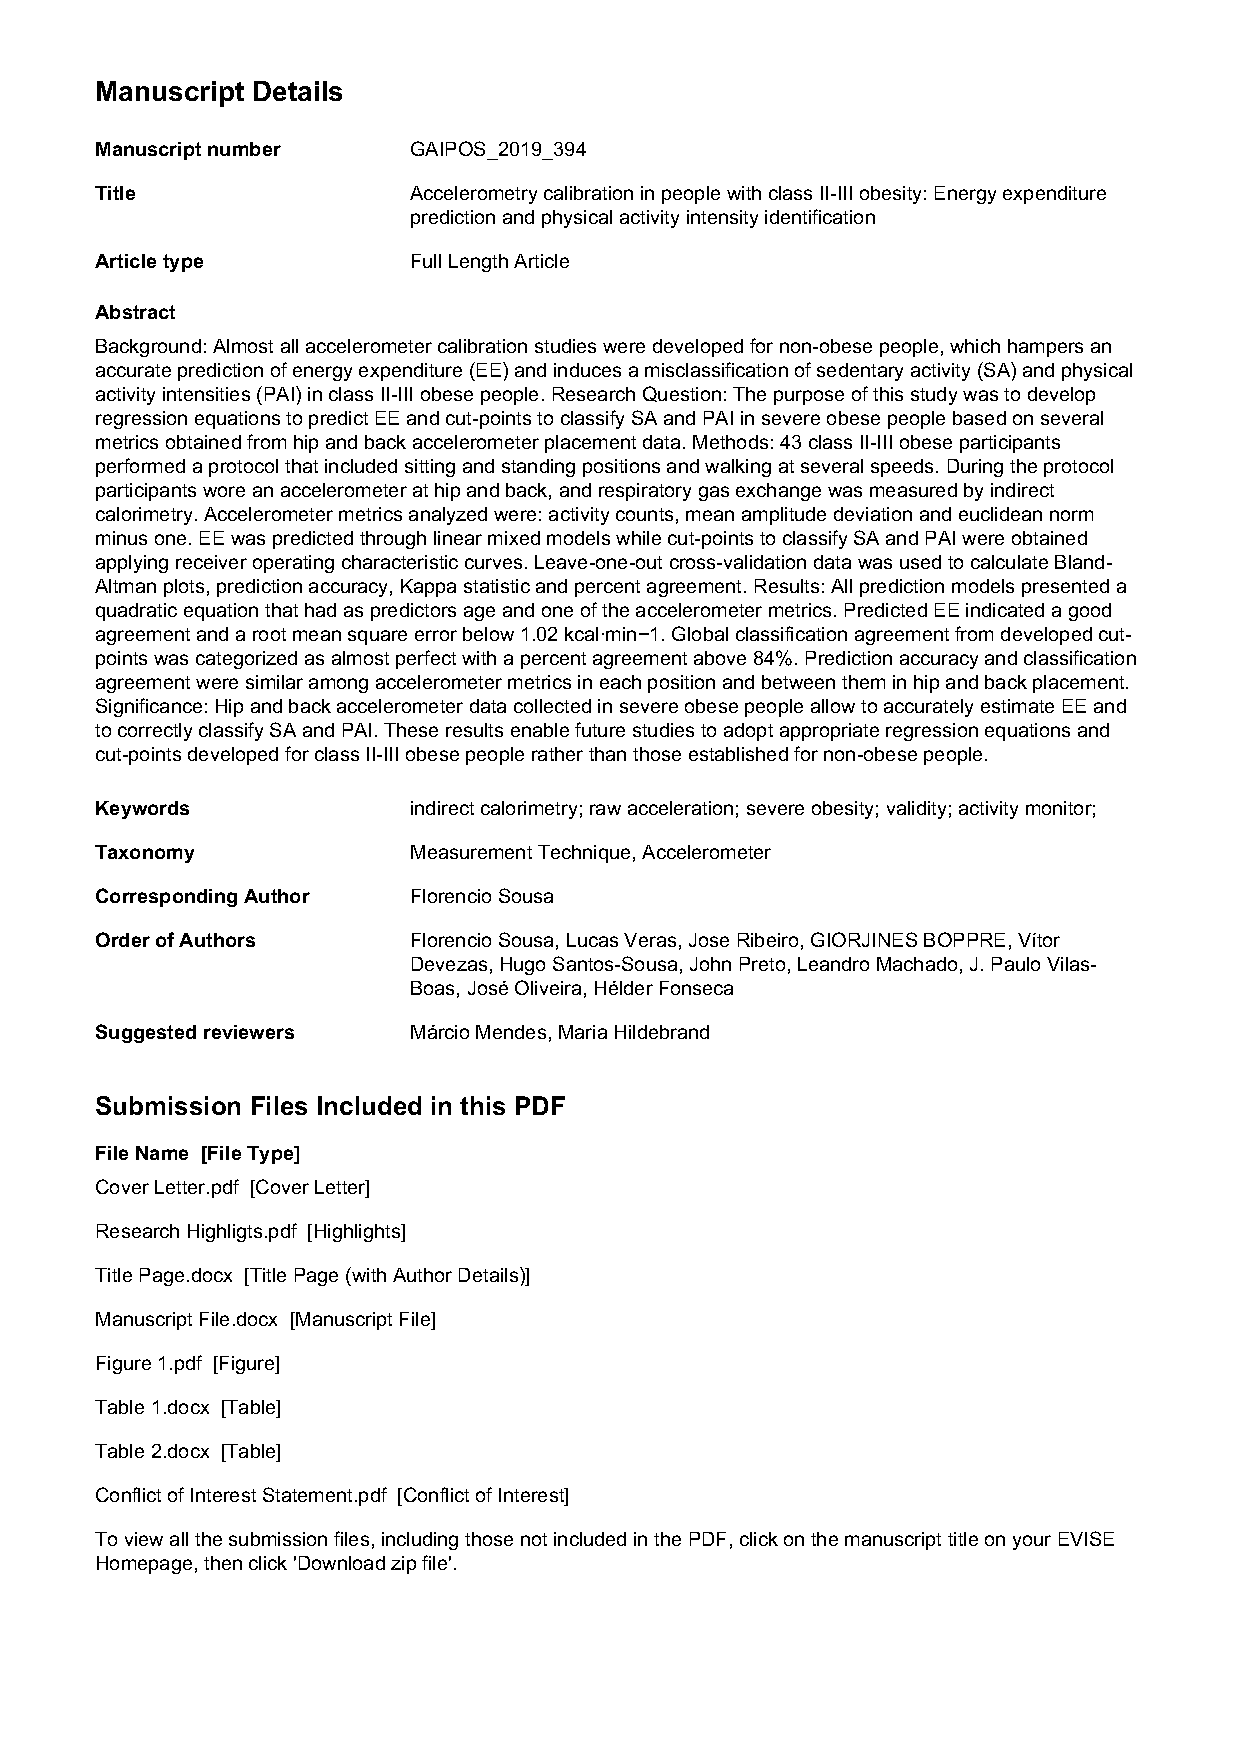
\includepdf[pages=-, pagecommand={}]{original_studies/Study_1.pdf}
\pagebreak

\section*{\vfill\raggedleft\bfseries Study 2}
\noindent \textbf{Accelerometer-based prediction of skeletal mechanical loading during walking in normal weight to severely obese subjects}
\addcontentsline{toc}{subsection}{3.2. Study 2 - Accelerometer-based prediction of skeletal mechanical loading during walking in normal weight to severely obese subjects}

\bigskip

\noindent Lucas Veras, Florêncio Diniz-Sousa, Giorjines Boppre, Vítor Devezas, Hugo Santos-Sousa, John Preto, Leandro Machado, João Paulo Vilas-Boas, José Oliveira, Hélder Fonseca
\pagebreak

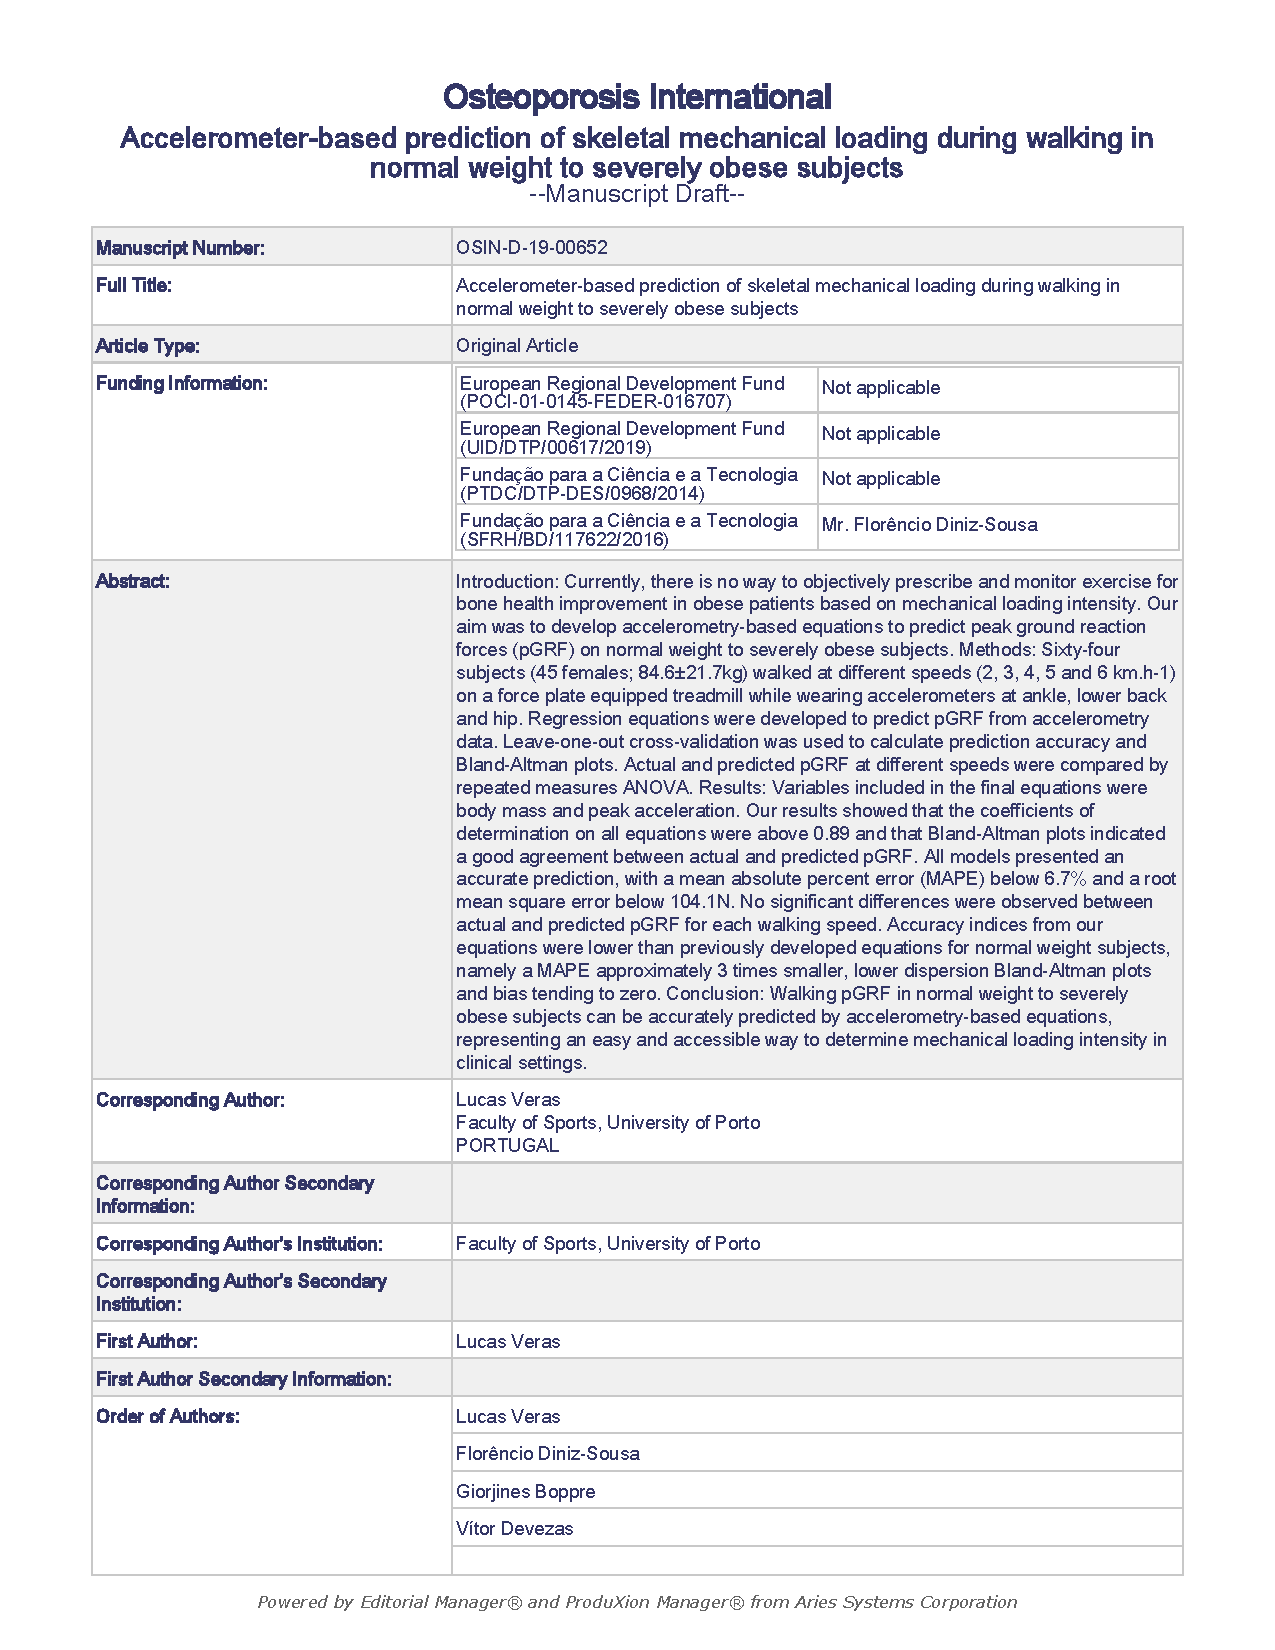
\includepdf[pages=-, pagecommand={}]{original_studies/Study_2.pdf}
\pagebreak

\end{document}